% Erstellt von Benjamin Thomitzni
% Version 1.0, 18.06.17
% 
% Für die Erstellung des Dokuments wurde eine Reihe an LaTeX Paketen verwendet. Diese sind unter der LPPL (http://www.latex-project.org/lppl.txt) Lizenz veröffentlich, falls nicht anders genannt.
%
%Ein Teil der Graphiken sind dem Splittermond Fanpaket von Meisterperson/Daniel Bruxmeier (https://meisterperson.wordpress.com/2015/02/24/splittermond-fanpaket/) entnommen. 
% Sie basieren auf Grafiken von Brenda Clarke (http://inadesign-stock.deviantart.com/art/Moody-Blues-Texture-Pack-1-261617011), Bethany Lerie (http://redlillith.deviantart.com/art/misc-tribal-brushes-14070868), Alex Ruiz (http://alexruizart.deviantart.com/art/Tribal-Tech-Photoshop-Brushes-414404973) & Carsten Jünger (http://pixelmixtur-stocks.deviantart.com/art/Wood-Texture-418149743)
% Das Fanlayout von Daniel Bruxmeier ist unter der CC-by 4.0 (http://creativecommons.org/licenses/by/4.0/deed.de) veröffentlicht worden. Texte und zusätzliche Illustrationen sind hiervon ausgenommen. 
%
%Das Splittermond Rollenspiel wird vom Uhrwerk-Verlag (http://www.uhrwerk-verlag.de/) vertrieben.
%
%Der Code compiliert mit pdflatex (https://www.ctan.org/pkg/pdftex)

\documentclass[12pt, a4paper, twoside, openany]{book}

\usepackage[utf8x]{inputenc} %https://www.ctan.org/pkg/inputenc
\usepackage{german} %Deutsche Sprache, https://www.ctan.org/pkg/german
\usepackage[]{graphicx} %Zusatzfunktionen für Graphiken, remove draft for release, https://www.ctan.org/pkg/graphicx
\usepackage{blindtext} %für lorem ipsum blindtext, https://www.ctan.org/pkg/blindtext
\usepackage{multicol} %für zweispaltig etc., https://www.ctan.org/pkg/multicol?lang=en
\usepackage[a4paper]{geometry} %Abstände innerhalb der Seiten, https://www.ctan.org/pkg/geometry
\geometry{
        a4paper,
        top=32mm,
        outer=13mm, 
        inner=29mm,
        footskip=0mm
}
\usepackage{float} %Float Optionen für Graphiken, https://www.ctan.org/pkg/float
%Header ------
\usepackage{fancyhdr} %Paket zum Einstellen des Headers, https://www.ctan.org/pkg/fancyhdr
\fancyhead{}
\fancyfoot{}
\fancyfoot[C]{\color{black} \Large  \textbf{\thepage}} %Fußnote, left even, right odd auf alternierenden Seiten Seitenzahl wechseln
\pagestyle{fancy}
\renewcommand{\headrulewidth}{0pt} % Ausschalten der Headerlinie
\renewcommand{\footrulewidth}{0pt}
%----- Farben
\usepackage{anyfontsize} %Größere/Kleinere Zeichen, https://www.ctan.org/pkg/anyfontsize
\usepackage[table]{xcolor} %Farben definierne können, table für rowcolor, https://www.ctan.org/pkg/xcolor
\definecolor{spmblue}{HTML}{25408F}%Überrschriftenfarbe
\definecolor{kastenblau}{HTML}{BADDF3}
\definecolor{kastenumrandung}{HTML}{5E9BD0}
\definecolor{spmback}{HTML}{ECF0F3}%Hintergrundfarbei
\definecolor{spmtabelle}{HTML}{ABE1FA}
\pagecolor{spmback}
%---- Veränderungen an den Überschriften
\usepackage{sectsty} %Kontrollieren von Chapter, Section Positon, https://www.ctan.org/pkg/sectsty

\allsectionsfont{\sffamily \centering} %Alle Überschriften zentrieren
\chapterfont{\sffamily \centering \color{spmblue}}
\subsectionfont{\sffamily \color{spmblue}\centering}
\subsubsectionfont{\sffamily \color{black}}

%---- Geometry paket um die margins einzustellen
\usepackage{authoraftertitle}%title, author und date einstellen und immer abrufen können, https://www.ctan.org/pkg/authoraftertitle, Public Domain Software Lizenz

%--- boxes
\usepackage{tcolorbox} %Farbige Box, https://www.ctan.org/pkg/tcolorbox
\usepackage{tikz} %Tikz, um zu zeichnen, https://www.ctan.org/pkg/pgf?lang=en, GNU Lizenz
\tcbuselibrary{skins}
%---- bessere auzählung
\usepackage{enumitem} %https://www.ctan.org/pkg/enumitem
\setlist{nosep} %oder \setlist{noitemsep}

%---- Metadaten
\title{Titel des Abenteuers}
\author{Autor}
\date{datum}
%----------------------
%Hintergrundeinstellungen
\usepackage{background}%Hintergründe einstellen, https://www.ctan.org/pkg/background
\backgroundsetup{
        scale=1,
        opacity=0.6,
        angle=0,
        contents={%Um gerade, ungerade zahl zu wechseln
                 \ifodd\value{page}
                         \includegraphics[width=\paperwidth]{bilder/Splittermond_Fanpaket/Hintergrund_links.png}
                 \else
                        \includegraphics[width=\paperwidth]{bilder/Splittermond_Fanpaket/Hintergrund_rechts.png}
                 \fi
                    }
               }
%------------
               \usepackage{lmodern}%Schrift, https://www.ctan.org/tex-archive/info/lmodern

%------ Margin für Chapter etc. oben verkleinern
               \usepackage{etoolbox} % https://www.ctan.org/pkg/etoolbox
\makeatletter
\patchcmd{\@makechapterhead}{50\p@}{0pt}{}{}
\patchcmd{\@makeschapterhead}{50\p@}{0pt}{}{}
\makeatother
\patchcmd{\chapter}{\thispagestyle{plain}}{\thispagestyle{fancy}}{}{}
%----- Defintion der Splittermond Box
\newtcolorbox{spmbox}[2][]{
            boxsep=5mm, 
            width=0.5\textwidth, 
            top=1mm, 
            bottom=1mm, 
            enhanced, 
            frame hidden, 
            interior style image=bilder/Splittermond_Fanpaket/Kasten_kurz.png
}


\begin{document}
\sffamily %Sans Serif Schriftart
\begin{titlepage}
    %Hintergrundbild für das Titelblatt
        \tikz[remember picture,overlay] \node[opacity=1,inner sep=0pt] at (current page.center){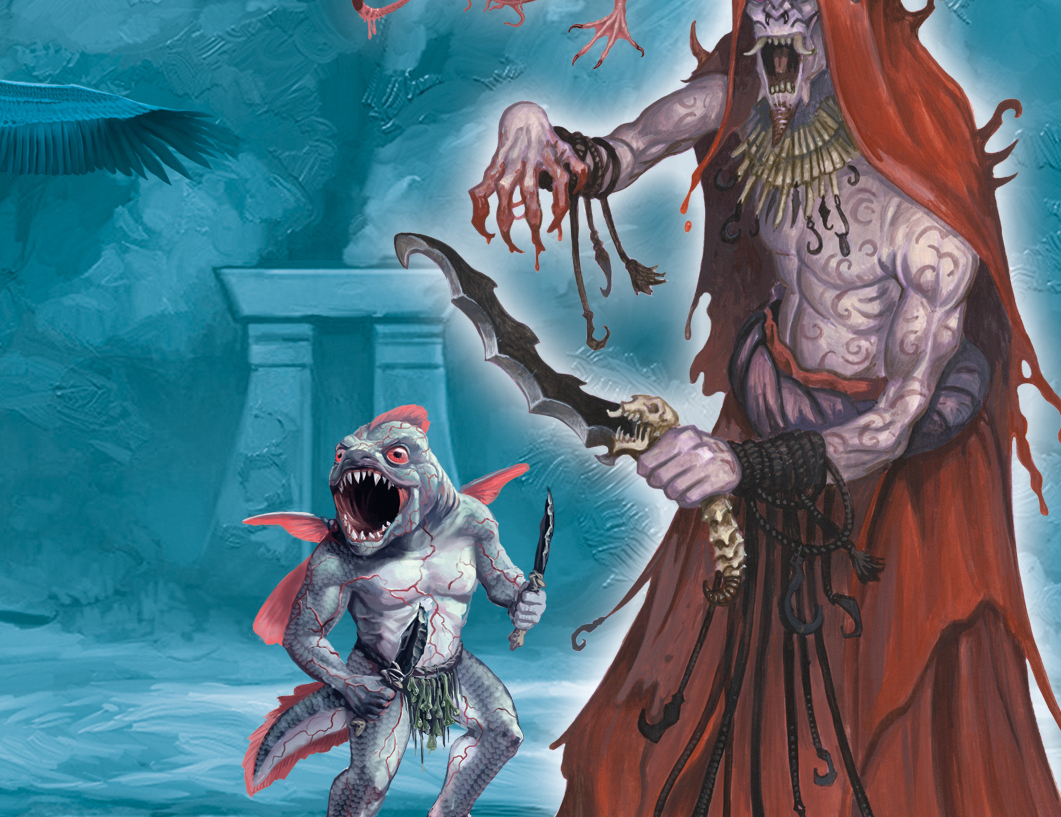
\includegraphics[height=\paperheight]{bilder/hintergrund.jpg}};
        %Balken auf der Seite des Titelblattes
        \tikz[remember picture,overlay] \node[opacity=1,inner sep=0pt] at (current page.center){
\includegraphics[width=\paperwidth,height=\paperheight]{bilder/Splittermond_Fanpaket/Coverbalken.png}};

        {
            \begin{center}
                    \color{white}
                    \fontsize{50}{60}
                    \selectfont
                    \textbf{\MyTitle}
            \end{center}
       }%Titelseite Block ende
    %Splittermond Fan Logo
       \begin{figure}[b]
               \centering
               
\includegraphics[scale=0.8]{bilder/Splittermond-Logo_fan_v2.png}
       \end{figure}
\end{titlepage}
\clearpage
{%Impressum und toc Seite

        {%Titel
            \begin{center}
                    \color{spmblue}
                    \fontsize{40}{50}
                    \selectfont
                    \textbf{\MyTitle}
            \end{center}
       }%Titel
    %Splittermond Fan Logo
       \begin{figure}[t]
               \centering
               
\includegraphics[scale=0.8]{bilder/Splittermond-Logo_fan_v2.png}
       \end{figure}
       
       \vfill
        \section*{Impressum}%* Versionen  da keine Nummern gewollt werden
        \addcontentsline{toc}{chapter}{Impressum}%Um zu Inhaltsverzeichnis hinzuzufügen
        \begin{center}
        Splittermond wird herausgegeben vom \textit{Uhrwerk}-Verlag.\\
        Bei diesem Werk handelt es sich um inoffizielles Fanmaterial.        
        \end{center}
        \subsection*{Autor}
        \begin{center} 
        \MyAuthor
        \end{center}
        \subsection*{Illustrationen}
        \begin{center}
        Max Mustermann        
        \end{center}

        \subsection*{Layout}
        \begin{center}
                Angelehnt an das Fanwerk Layoutvorlage von Daniel Bruxmeier unter Verwendung von Graphiken aus seinem Splittermond Fanpaket,\\ erstellt in \LaTeX ~und compiliert mit \textit{pdflatex} von Benjamin Thomitzni. \\
        Basierend auf Graphiken von \\ 
        Brenda Clarke, Buthany Lerie, Alex Ruiz und Carsten Jünger         
        \end{center}
        \subsection*{Lizenz}
        \begin{center}
                \tiny
                Dieses Layout steht unter der \textit{Creative-Commens}-Lizenz. \\
                
\includegraphics[scale=1]{bilder/Splittermond_Fanpaket/CC-BY.png}\\
                Dies umfasst ausdrücklich nicht die eigentlichen Inhalte des Dokuments wie Texte oder zusätzliche Illustrationen. \\
                Bei Nutzung diess Layout bitte wenn möglich das endgültige Werk ebenfalls unter einer \textit{Creatives-Commens}-Lizenz stellen. 
        \end{center}
}
%---------- Inhaltsverzeichnis
        \tableofcontents
%----------
\chapter*{\MyTitle}
        \addcontentsline{toc}{chapter}{\MyTitle}

\begin{multicols}{2}
        \subsubsection*{von \MyAuthor}
        Blindtext blabla
        \begin{spmbox}
                {\begin{center}
                    \color{spmblue}
                    \Large
                    \textbf{\MyTitle}
                \end{center}}
             Zusammenfassung des Abenteuers. Text. Blablabla. \\
                \textbf{Region:} Wo auch immer\\
                \textbf{Schauplätze:} In einer Stadt\\
                \textbf{Erfahrung:} Heldengrad X\\
                \textbf{Zeitraum:} 2-999 Tage\\
        \end{spmbox}
        \subsection*{Hintergrund}
            \Blindtext[1][1]
        \subsection*{Handlung}
            \Blindtext[1][1]
        \subsection*{Auswahl der Abenteuerer}
            Irgendwelche Idioten die sterben wollen.             
\end{multicols}
\section*{Einstieg: Wer, Wie, Wo, Was, Wie, Hä?}
\addcontentsline{toc}{section}{Einstieg: Wer, Wie, Wo, Was, Wie, Hä?}
\begin{multicols}{2}
        \Blindtext[1][1]
        \begin{enumerate}[label=\textbullet]
                \item Ein Item der Liste
                \item Ein Zweites Item auf der Liste

        \end{enumerate}

\subsection*{Nummer Eins}
\Blindtext[1][1]
\subsubsection*{Unterüberschrift}
\Blindtext[1][1]
{
\begin{center}

\includegraphics[width=0.5\textwidth]{bilder/foo.png}
\end{center}
}
\end{multicols}
\begin{figure}[H]
        \centering
        
\includegraphics[width=.6\textwidth]{bilder/foo.png}
        \label{fig:piel}
\end{figure}

\begin{multicols}{2}
        \Blindtext[1][1]
        
       \vbox{%Gegner Block
                {
                \vspace{5mm}
                \Large
                \textbf{Beispielgegner}
                }\\
                \rule{0.5\textwidth}{0.2em}\\
                \resizebox{0.5\textwidth}{!}{%Automatisches Skalieren der Tabelle
                \begin{tabular}{c|c|c|c|c|c|c|c}
                        \rowcolor{spmtabelle}
                        \textbf{AUS} & \textbf{BEW} & \textbf{INT} & \textbf{KON} & \textbf{MYS} & \textbf{STÄ} & \textbf{VER} & \textbf{WIL} \\
                        1            & 1            & 1            & 1            & 1            & 1            & 1            & 1            \\
                        \rowcolor{spmtabelle}
                        \textbf{GK}  & \textbf{GSW} & \textbf{LP}  & \textbf{FO}  & \textbf{VTD} & \textbf{SR}  & \textbf{KW}  & \textbf{GW}  \\
                        1            & 1            & 1            & 1            & 1            & 1            & 1            & 1           
        \end{tabular}}\\ 
        \resizebox{0.5\textwidth}{!}{
                \begin{tabular}{l|c|c|c|c|c}
                        \rowcolor{spmtabelle}
                        \textbf{Waffe} & \textbf{Wertf} & \textbf{Schaden} & \textbf{WGS} & \textbf{INI} & \textbf{Merkmale} \\
                        Körper         &            9   & 1W6              & 6 Ticks      & 7-1W6        & \\ 

        \end{tabular}
        }%Resizebox
        \vspace{2mm}\\
        \textbf{Typus:} Humanoid \\
        \textbf{Monstergrad:} 0/0 \\
        \textbf{Fertigkeiten:} Absolut Nix 1, Nix 2 \\
        \textbf{Meisterschaften:} Bäcker (Handwerk) \\
        \textbf{Merkmale:} Dämmersicht \\
        \textbf{Beute:} Lollipop \\
        \rule{0.5\textwidth}{0.2em}\\
        \vspace{5mm}
        }%Gegner Block Ende
\end{multicols}    
\end{document}

